\section{Design and Implementation}
\subsection{Power Stage Calculation and Component Selection}
Design of a 1000W Push-Pull Converter Operating in Continuous Conduction Mode (CCM) with
the following specifications:
\begin{table}[h!]
    \centering
    \begin{tabular}{ll}
        \toprule
        \textbf{Parameter} & \textbf{Value} \\
        \midrule
        Input Voltage ($V_{\text{in}}$) & $\SI{310}{\volt}$ \\
        Duty Cycle ($D$) & $30\% $ \\
        Output Voltage ($V_{\text{out}}$) & $\SI{24}{\volt}$ \\
        Diode Voltage $(V_d)$ & $1V$\\
        Output Power ($P_{\text{out}}$) & $\SI{1000}{\watt}$ \\
        Switching Frequency ($f_{\text{sw}}$) & $\SI{100}{\kilo\hertz}$ \\
        Ripple Current Rated ($\Delta I_{\text{ripple}}$) & $30\%$ \\
        Ripple Voltage Rated ($\Delta V_{\text{ripple}}$) & $1\%$ \\
        Efficiency & $90\%$ \\
        \bottomrule
    \end{tabular}
    \caption{Input Parameters}
    \label{tab:system_parameters}
\end{table}
\subsection{Power Stage Calculation}

\subsubsection*{Transformer Turns Ratio (\(T\))}
\begin{equation}
T = \frac{2 \cdot V_{\text{in}} \cdot D}{V_{\text{out}} + 2 \cdot V_d} = \frac{2 \cdot 310 \cdot 0.3}{24 + 2 \cdot 1} = \boxed{7.15}
\end{equation}

\subsubsection*{Output Current (\(I_{\text{out}}\))}
\begin{equation}
I_{\text{out}} = \frac{P_{\text{out}}}{V_{\text{out}}} = \frac{500}{24} = \boxed{\SI{20.83}{\ampere}}
\end{equation}

\subsubsection*{Load Resistance (\(R_L\))}
\begin{equation}
R_L = \frac{V_{\text{out}}^2}{P_{\text{out}}} = \frac{24^2}{500} = \boxed{\SI{1.152}{\ohm}}
\end{equation}

\subsubsection*{Input Power (\(P_{\text{in}}\))}
\begin{equation}
P_{\text{in}} = \frac{P_{\text{out}}}{\eta} = \frac{500}{0.9} = \boxed{\SI{555.56}{\watt}}
\end{equation}

\subsubsection*{Primary Average Current (\(I_{\text{p\_avg}}\))}
\begin{equation}
I_{p\_avg} = \frac{P_{in}}{2 \cdot V_{in}} = \frac{1111.11}{2 \cdot 310} = \boxed{1.792\;\text{A}} 
\end{equation}

\subsubsection*{Primary Ripple Current (\(\Delta I_{\text{p}}\))}
\begin{equation}
\Delta I_p = \text{Ripple\_I} \cdot I_{p\_avg} = 0.3 \cdot 1.792 = \boxed{0.538\;\text{A}}
\end{equation}

\subsubsection*{Primary Inductance (\(L_p\))}
\begin{equation}
L_p = \frac{V_{in} \cdot D}{F_{sw} \cdot \Delta I_p} = \frac{310 \cdot 0.3}{100 \times 10^3 \cdot 0.538} = \boxed{1.73\;\text{mH}}
\end{equation}

\subsubsection*{Secondary Inductance (\(L_s\))}
\begin{equation}
L_s = \frac{L_p}{T^2} = \frac{1.73 \times 10^{-3}}{(7.15)^2} = \boxed{33.9\;\mu\text{H}}
\end{equation}

\subsubsection*{Secondary Voltage (\(V_s\))}
\begin{equation}
V_s = \frac{V_{\text{in}}}{T} = \frac{310}{7.15} = \boxed{\SI{43.36}{\volt}}
\end{equation}

\subsubsection*{Output Ripple Current (\(\Delta I_{\text{out}}\))}
\begin{equation}
\Delta I_{out} = \text{Ripple\_I} \cdot I_{out} = 0.3 \cdot 41.67 = \boxed{12.5\;\text{A}}
\end{equation}

\subsubsection*{Output Maximum Current}
\begin{equation}
I_{out\_max} = I_{out} + \frac{\Delta I_{out}}{2} = 41.67 + 6.25 = \boxed{47.92\;\text{A}} \\
\end{equation}

\subsubsection*{Output Minimum Current}
\begin{equation}
I_{out\_min} = I_{out} - \frac{\Delta I_{out}}{2} = 41.67 - 6.25 = \boxed{35.42\;\text{A}}
\end{equation}

\subsubsection*{Output Inductance (\(L_{\text{out}}\))}
\begin{equation}
L_{out} = \frac{V_{out} \cdot (1 - 2D)}{F_{sw} \cdot \Delta I_{out}} = \frac{24 \cdot 0.4}{100 \times 10^3 \cdot 12.5} = \boxed{7.68\;\mu\text{H}}
\end{equation}

\subsubsection*{Output Ripple Voltage (\(\Delta V_{\text{out}}\))}
\begin{equation}
\Delta V_{\text{out}} = \text{Ripple\_V} \cdot V_{\text{out}} = 0.01 \cdot 24 = \boxed{\SI{0.24}{\volt}}
\end{equation}

\subsubsection*{Output Capacitor (\(C_{\text{out}}\))}
\begin{equation}
C_{out} = \frac{\Delta I_{out}}{8 \cdot F_{sw} \cdot \Delta V_{out}} = \frac{12.5}{8 \cdot 100 \times 10^3 \cdot 0.24} = \boxed{65.1\;\mu\text{F}}
\end{equation}
\subsubsection*{MOSFET Selection}
\begin{center}
    \begin{minipage}{0.4\textwidth}
        \centering
        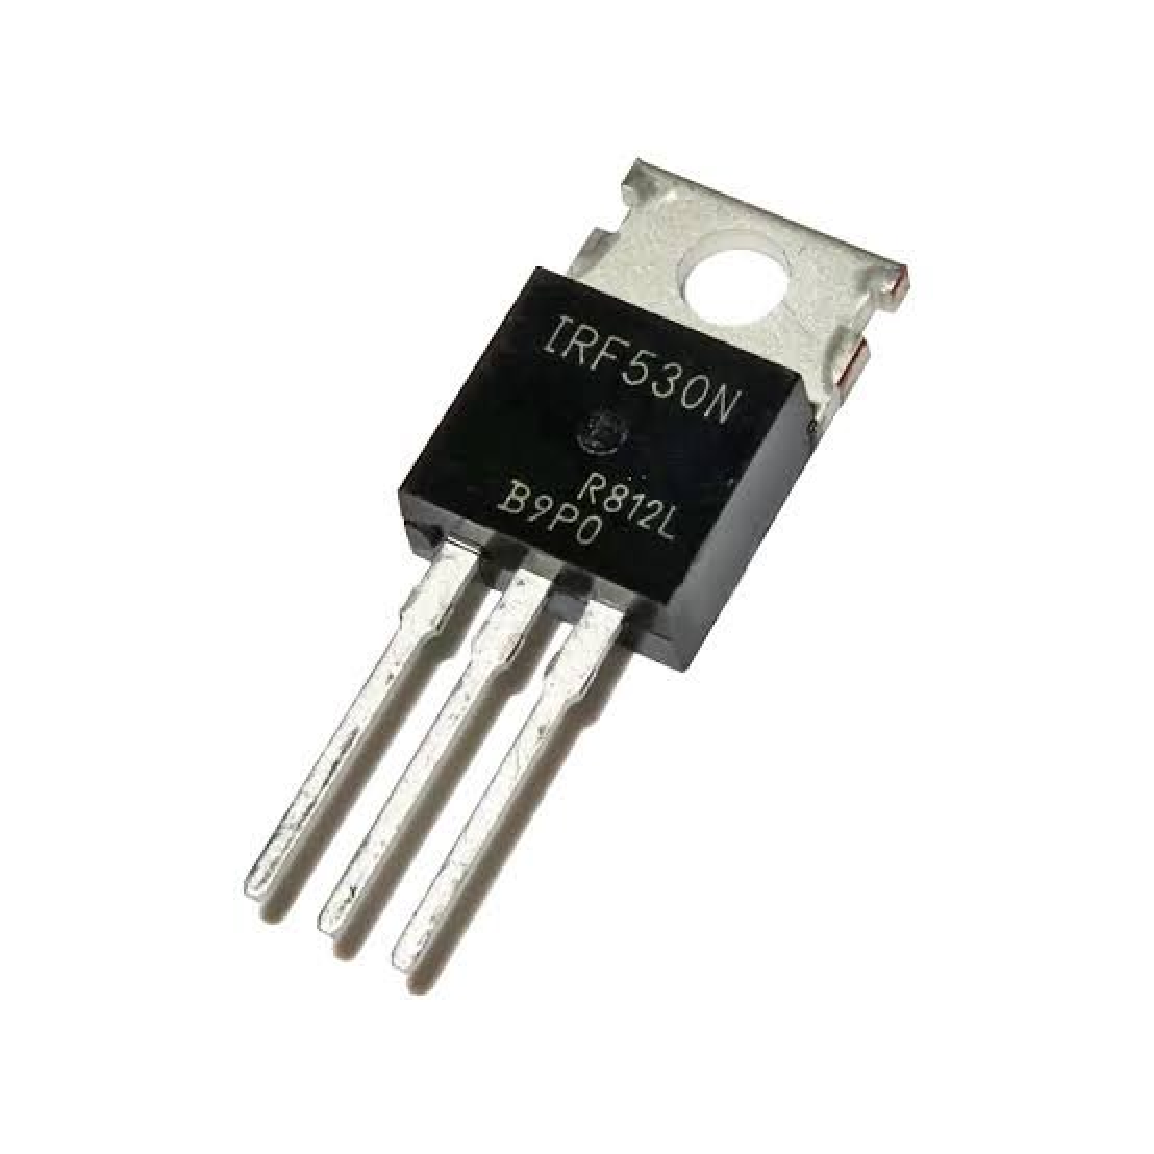
\includegraphics[width=0.8\linewidth]{Pictures/pics/mosfet.pdf} % Replace with your image file
        %\captionof{figure}{This is a figure.} % Add a caption
    \end{minipage}
    \hfill % Adds space between the minipages
    \begin{minipage}{0.55\textwidth}
    \centering
    \captionof{table}{STW11NM80 MOSFET}
    \label{tab:IRF530}
    \begin{tabular}{lcc}
    \toprule
    \footnotesize
    \textbf{Parameter} & \textbf{Value} & \textbf{Test Conditions} \\
    \midrule
     $V_{DS}$ & \SI{800}{\volt} & Absolute Maximum Rating \\
     $I_D$ & \SI{15}{\ampere} & $T_C = \SI{25}{\celsius}$ \\
     & \SI{10}{\ampere} & $T_C = \SI{100}{\celsius}$ \\
     $R_{DS(on)}$ & \SI{0.16}{\ohm} & $V_{GS} = \SI{10}{\volt}, I_D = \SI{8.4}{\ampere}$ \\
    \bottomrule
    \end{tabular}
    \end{minipage}
\end{center}
\subsubsection*{Diode Selection}
\begin{center}
    \begin{minipage}{0.4\textwidth}
        \centering
        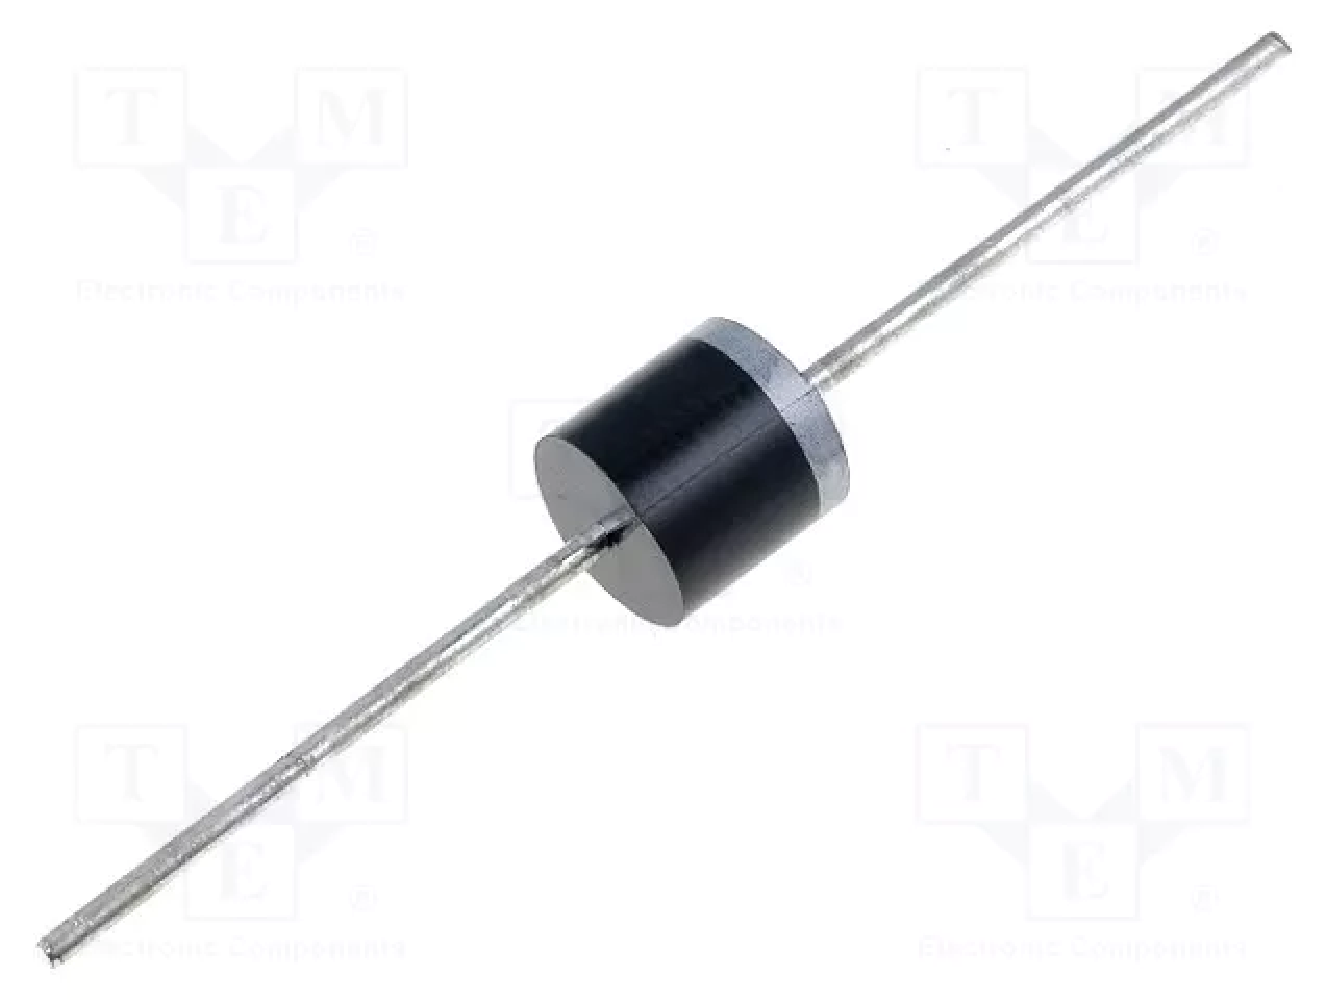
\includegraphics[width=0.7\linewidth]{Pictures/pics/diode.pdf} % Replace with your image file
        %\captionof{figure}{This is a figure.} % Add a caption
    \end{minipage}
    \hfill % Adds space between the minipages
    \begin{minipage}{0.55\textwidth}
    \centering
    \captionof{table}{VS-E5PX6012 Diode}
        \label{tab:SR510}
        \begin{tabular}{lcc}
        \toprule
        \textbf{Parameter} & \textbf{Value} & \textbf{Test Conditions} \\
        \midrule
        $V_{RRM}$ & \SI{1000}{\volt} & Maximum repetitive rating \\
        $I_F$ & \SI{50}{\ampere} & Continuous, $T_A = \SI{25}{\celsius}$ \\
        \bottomrule
        \end{tabular}
    \end{minipage}
\end{center}
\subsection{Transformer Design}
\begin{table}[h!]
\centering
\caption{Input Parameters for Transformer Design}
\begin{tabular}{llll}
\toprule
\textbf{Parameter} & \textbf{Value} & \textbf{Parameter} & \textbf{Value} \\ \midrule
$P_{\text{out}}$ & $\SI{1000}{\watt}$ & $K_f$ & $4$ \\
$V_{\text{in}}$ & $\SI{310}{\volt}$ & $B_m$ & $\SI{0.05}{\tesla}$ \\
$U$ & $1.41$ & $F_{\text{sw}}$ & $\SI{100e3}{\hertz}$ \\
$n$ & $0.9$ & $\alpha$ & $0.5$ \\
$K_u$ & $0.4$ & $D$ & $0.3$ \\
$I_{\text{out}}$ & $\SI{20.83}{\ampere}$ & & \\ \bottomrule
\end{tabular}
\end{table}
\subsubsection*{Secondary Apparent Power (\(P_t\))}
\begin{equation}
P_t = \left(\frac{P_{out}}{\eta}\right) \cdot U + P_{out} \cdot U 
    = \left(\frac{1000}{0.9}\right) \cdot 1.41 + 1000 \cdot 1.41 
    = \boxed{2976.67\;\text{VA}}
\end{equation}


\subsubsection*{Electrical Condition (\(K_e\))}
\begin{equation}
K_e = 0.145 \cdot K_f^2 \cdot F_{sw}^2 \cdot B_m^2 \cdot 10^{-4} 
    = 0.145 \cdot (4)^2 \cdot (100 \times 10^3)^2 \cdot (0.05)^2 \cdot 10^{-4} 
    = \boxed{5800}
\end{equation}

\subsubsection*{Core Geometry (\(K_g\))}
\begin{equation}
K_g = \left(\frac{P_t}{2 \cdot K_e \cdot \alpha}\right) \cdot 1.35 
    = \left(\frac{2976.67}{2 \cdot 5800 \cdot 0.5}\right) \cdot 1.35 
    = \boxed{0.6928\;\text{cm}^5}
\end{equation}

\begin{figure}[h!]
    \centering
    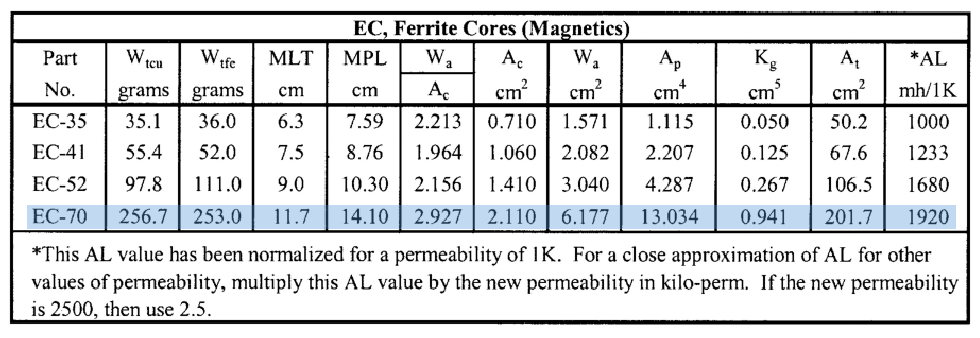
\includegraphics[width=1\linewidth]{Pictures/images/EC-70_table.pdf}
    \caption{\textcolor{blue}{\textit{\footnotesize EC Core Parameter Table List}}}
\end{figure} 
\newpage
\begin{figure}[h!]
    \centering
    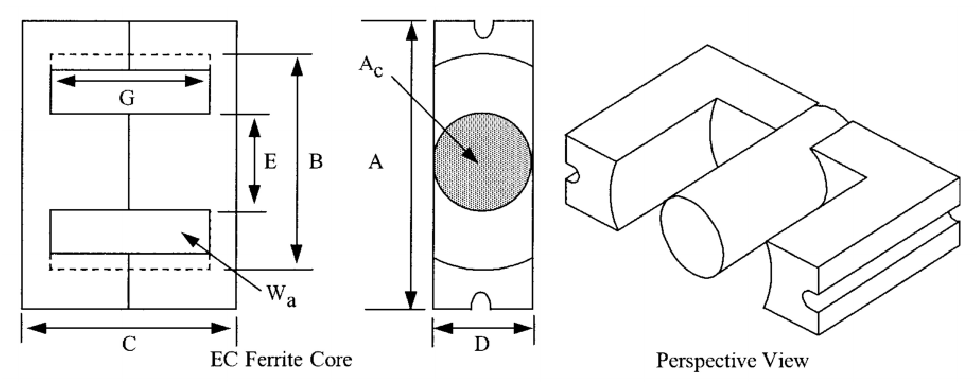
\includegraphics[width=1\linewidth]{Pictures/images/EC-70_structure.pdf}
    \caption{\textcolor{blue}{\textit{\footnotesize EC-70 Core}}}
\end{figure} 


\begin{table}[h!]
\centering
\caption{Core Parameters for Transformer Design}
\begin{tabular}{llll}
\toprule
\textbf{Parameter} & \textbf{Value} & \textbf{Parameter} & \textbf{Value} \\ \midrule
MPL & $\SI{14.10}{\centi\meter}$ & We & $\SI{253}{\gram}$ \\
MLT & $\SI{11.7}{\centi\meter}$ & $A_c$ & $\SI{2.11}{\centi\meter\squared}$ \\
$W_a$ & $\SI{6.1777}{\centi\meter\squared}$ & $A_p$ & $\SI{13.034}{\centi\meter\tothe{4}}$ \\
$K_{\text{gs}}$ & $\SI{0.0941}{\centi\meter\tothe{5}}$ & & \\ \bottomrule
\end{tabular}
\end{table}

\subsubsection*{Current Density (\(J\))}
\begin{equation}
J = \frac{P_t \cdot 10^4}{K_f \cdot K_u \cdot B_m \cdot F_{sw} \cdot A_p} 
  = \frac{2976.67 \cdot 10^4}{4 \cdot 0.4 \cdot 0.05 \cdot 100 \times 10^3 \cdot 13.034} 
  = \boxed{285.5\;\frac{\text{A}}{\text{cm}^2}}
\end{equation}

\subsubsection*{Primary Turns (\(N_p\))}
\begin{equation}
N_p = \frac{V_{in} \cdot 10^4}{K_f \cdot B_m \cdot F_{sw} \cdot A_c} 
    = \frac{310 \cdot 10^4}{4 \cdot 0.05 \cdot 100 \times 10^3 \cdot 2.11} 
    = \boxed{73.5\;\text{turns}}
\end{equation}

\subsubsection*{Input Current (\(I_{in}\))}
\begin{equation}
I_{in} = \frac{P_{out}}{\eta \cdot V_{in}} 
       = \frac{1000}{0.9 \cdot 310} 
       = \boxed{3.584\;\text{A}}
\end{equation}

\subsubsection*{Primary Bare Wire Area (\(A_{pw}\))}
\begin{equation}
A_{pw} = \frac{I_{in} \cdot \sqrt{D}}{J} 
       = \frac{3.584 \cdot \sqrt{0.3}}{285.5} 
       = \boxed{6.88\;\text{mm}^2}
\end{equation}

\subsubsection*{Secondary Voltage}
\begin{equation}
    V_s = \frac{V_{\text{in}}}{7.15} = \frac{310}{7.15} \approx \boxed{43.36\,\text{V}}
\end{equation}

\subsubsection*{Secondary  Turn \( N_s\)}
\begin{equation}
    N_s = \left( \frac{N_p \cdot V_s}{V_{\text{in}}} \right) \cdot \left( 1 + \frac{\alpha}{100} \right) = \left( \frac{89 \cdot 43.36}{310} \right) \cdot 1.005 = \approx \boxed{13.5\,\text{turns}}
\end{equation}

\subsubsection*{Secondary Wire Area}
\begin{equation}
A_{\text{sw}} = \frac{I_{\text{out}} \cdot \sqrt{D}}{J} 
= \frac{41.67 \cdot \sqrt{0.3}}{383.4}
\approx \boxed{0.08\,\text{cm}^2}
\end{equation}

\subsection{Output Inductor Design}
\begin{table}[h!]
\centering
\caption{Input Parameters for Ferrite Core Selection}
\begin{tabular}{ll}
\toprule
\textbf{Parameter} & \textbf{Value} \\ \midrule
Inductance (\(L\)) & \(\SI{16e-6}{\henry}\) \\
DC Current (\(I_o\)) & \(\SI{20.83}{\ampere}\) \\
AC Ripple Current (\(\Delta I\)) & \(\SI{6.25}{\ampere}\) \\
Output Power (\(P_o\)) & \(\SI{500}{\watt}\) \\
Regulation (\(\alpha\)) & \(1\%\) \\
Switching Frequency (\(F_s\)) & \(\SI{100e3}{\hertz}\) \\
Flux Density (\(B_m\)) & \(\SI{0.25}{\tesla}\) \\
Window Utilization (\(K_u\)) & \(0.4\) \\
Temperature Rise (\(T_r\)) & \(\SI{25}{\celsius}\) \\ \bottomrule
\end{tabular}
\end{table}

\subsubsection*{Peak Current}
\begin{equation}
\text{(\(I_{\text{pk}}\))} = I_o + \frac{\Delta I}{2} = 20.83 + \frac{6.25}{2} = \boxed{\SI{23.96}{\ampere}}
\end{equation}

\subsubsection*{Energy Handling}
\begin{equation}
\text{ (\(E\))} = \frac{1}{2} L I_{\text{pk}}^2 = \frac{1}{2} \cdot 16 \times 10^{-6} \cdot (23.96)^2 = \boxed{\SI{0.00459}{\joule}}
\end{equation}

\subsubsection*{Electrical Coefficient}
\begin{equation}
\text{ (\(K_e\))} = 0.145 \cdot P_o \cdot B_m^2 \cdot 10^{-4} 
= 0.145 \cdot 500 \cdot (0.25)^2 \cdot 10^{-4}
= \boxed{0.000453}
\end{equation}

\subsubsection*{Core Geometry}
\begin{equation}
K_g = \frac{E^2}{K_e \cdot \alpha} = \frac{(0.00459)^2}{0.000453 \cdot 1} = \boxed{\SI{0.0465}{\centi\meter\tothe{5}}}
\end{equation}

\begin{figure}[h!]
    \centering
    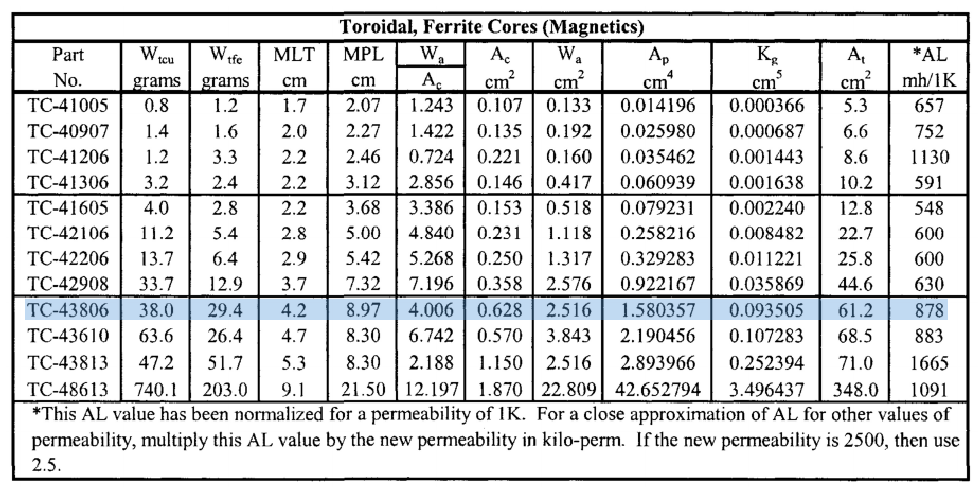
\includegraphics[width=1\linewidth]{Pictures/images/toroidal_core_table.pdf}
    \caption{\textcolor{blue}{\textit{\footnotesize Toroidal Core Parameter Table List}}}
\end{figure} 
\begin{figure}[h!]
    \centering
    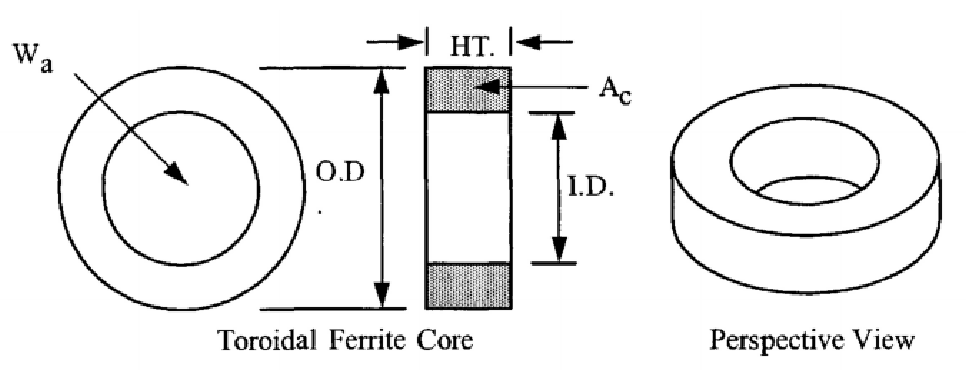
\includegraphics[width=1\linewidth]{Pictures/images/inductor_core_structure.pdf}
    \caption{\textcolor{blue}{\textit{\footnotesize TC-43806 Core}}}
\end{figure} 
\subsubsection*{Current Density}
\begin{equation}
J = \frac{2 \cdot E \cdot 10^4}{B_m \cdot A_p \cdot K_u} 
  = \frac{2 \cdot 0.00884 \cdot 10^4}{0.25 \cdot 1.5803 \cdot 0.4} 
  = \boxed{1119\;\frac{\text{A}}{\text{cm}^2}}
\end{equation}

\subsubsection*{RMS Current}
\begin{equation}
I_{rms} = \sqrt{I_o^2 + \Delta I^2} 
        = \sqrt{(41.67)^2 + (12.5)^2} 
        = \boxed{43.5\;\text{A}}
\end{equation}

\subsubsection*{Bare Wire Area}
\begin{equation}
A_w = \frac{I_{rms}}{J} 
    = \frac{43.5\;\text{A}}{1119\;\frac{\text{A}}{\text{cm}^2}}
    = \boxed{0.0389\;\text{cm}^2}
\end{equation}

\subsubsection*{Selected Wire Area}
\[
A_{ws} = 0.04\ \text{cm}^2
\]

\subsubsection*{Effective Window Area}
\begin{itemize}
    \item $S_3 = 0.75$ Window Effective factor for Ferrite core
\end{itemize}
\begin{equation}
W_{aeff} = W_a \cdot S_3 
         = 2.516\;\text{cm}^2 \cdot 0.75 
         = \boxed{1.887\;\text{cm}^2}
\end{equation}

\subsubsection*{Number of Turn}
\begin{itemize}
    \item $S_2 = 0.6$ Fill Factor 
\end{itemize}
\begin{equation}
N = \frac{W_{aeff} \cdot S_2}{A_{ws}} 
  = \frac{1.887\;\text{cm}^2 \cdot 0.6}{0.04\;\text{cm}^2} 
  = \boxed{28.3\;\text{turns}} \quad (\text{Round to } 28\;\text{turns})
\end{equation}

\subsubsection*{Required Air Gap}
\begin{equation}
L_g = \frac{0.4 \pi N^2 A_c \cdot 10^{-8}}{L} - \frac{MPL}{\mu_0} 
    = \frac{0.4 \pi \cdot 28^2 \cdot 0.628 \cdot 10^{-8}}{7.7 \times 10^{-6}} - \frac{8.97}{2500} 
    = \boxed{0.8\;\text{mm}}
\end{equation}

\newpage
\subsection{Simulation On LTspice}
\begin{figure}[h!]
    \centering
    
\includegraphics[width=0.9\linewidth]{Pictures/images/schem.pdf}
    \caption{\textcolor{blue}{\textit{\footnotesize Push-Pull Converter Schematic on LTspice}}}
\end{figure}

\begin{figure}[h!]
    \centering
    
\includegraphics[width=0.8\linewidth]{Pictures/images/output_voltage.pdf}
    \caption{\textcolor{blue}{\textit{\footnotesize Output Voltage Waveform}}}
\end{figure}

\begin{figure}[h!]
    \centering
    
\includegraphics[width=0.8\linewidth]{Pictures/images/output_current.pdf}
    \caption{\textcolor{blue}{\textit{\footnotesize Output Current Waveform}}}
\end{figure}

\newpage
\begin{figure}[h!]
    \centering
    
\includegraphics[width=0.8\linewidth]{Pictures/images/inductor_current.pdf}
    \caption{\textcolor{blue}{\textit{\footnotesize  Secondary Voltage and Inductor Current Waveform}}}
\end{figure}

\begin{figure}[h!]
    \centering
    
\includegraphics[width=0.8\linewidth]{Pictures/images/duty_s1_s2.pdf}
    \caption{\textcolor{blue}{\textit{\footnotesize Duty Cycle of S1 and S2}}}
\end{figure}
